%
% introduction.tex
%
% Copyright (C) 2022 by Universidade Federal de Santa Catarina.
%
% GNSS Networks Based on Small Satellites
%
% This work is licensed under the Creative Commons Attribution-ShareAlike 4.0
% International License. To view a copy of this license,
% visit http://creativecommons.org/licenses/by-sa/4.0/.
%

%
% \brief Introduction chapter.
%
% \author Gabriel Mariano Marcelino <gabriel.mm8@gmail.com>
%
% \version 0.0.0
%
% \date 2019/11/30
%

\chapter{Introduction} \label{ch:introduction}

Este trabalho tem como proposta o estudo, verificação de viabilidade e implementação de uma rede de um Sistema Global de Navegação por Satélite (\textit{Global Navigation Satellite System}, GNSS\nomenclature{\textbf{GNSS}}{Global Navigation Satellite System.}) baseada em satélites de pequeno porte, considerando especialmente os nanossatélites, ou em específico os CubeSats.

Os satélites de pequeno porte vêm crescendo de forma exponencial nos últimos anos, como pode ser visto na \autoref{fig:cubesat-launches} onde têm-se o número de lançamentos anuais de nanossatélites desde 1998, e o número previsto até 2025.

\begin{figure}[!ht]
    \begin{center}
        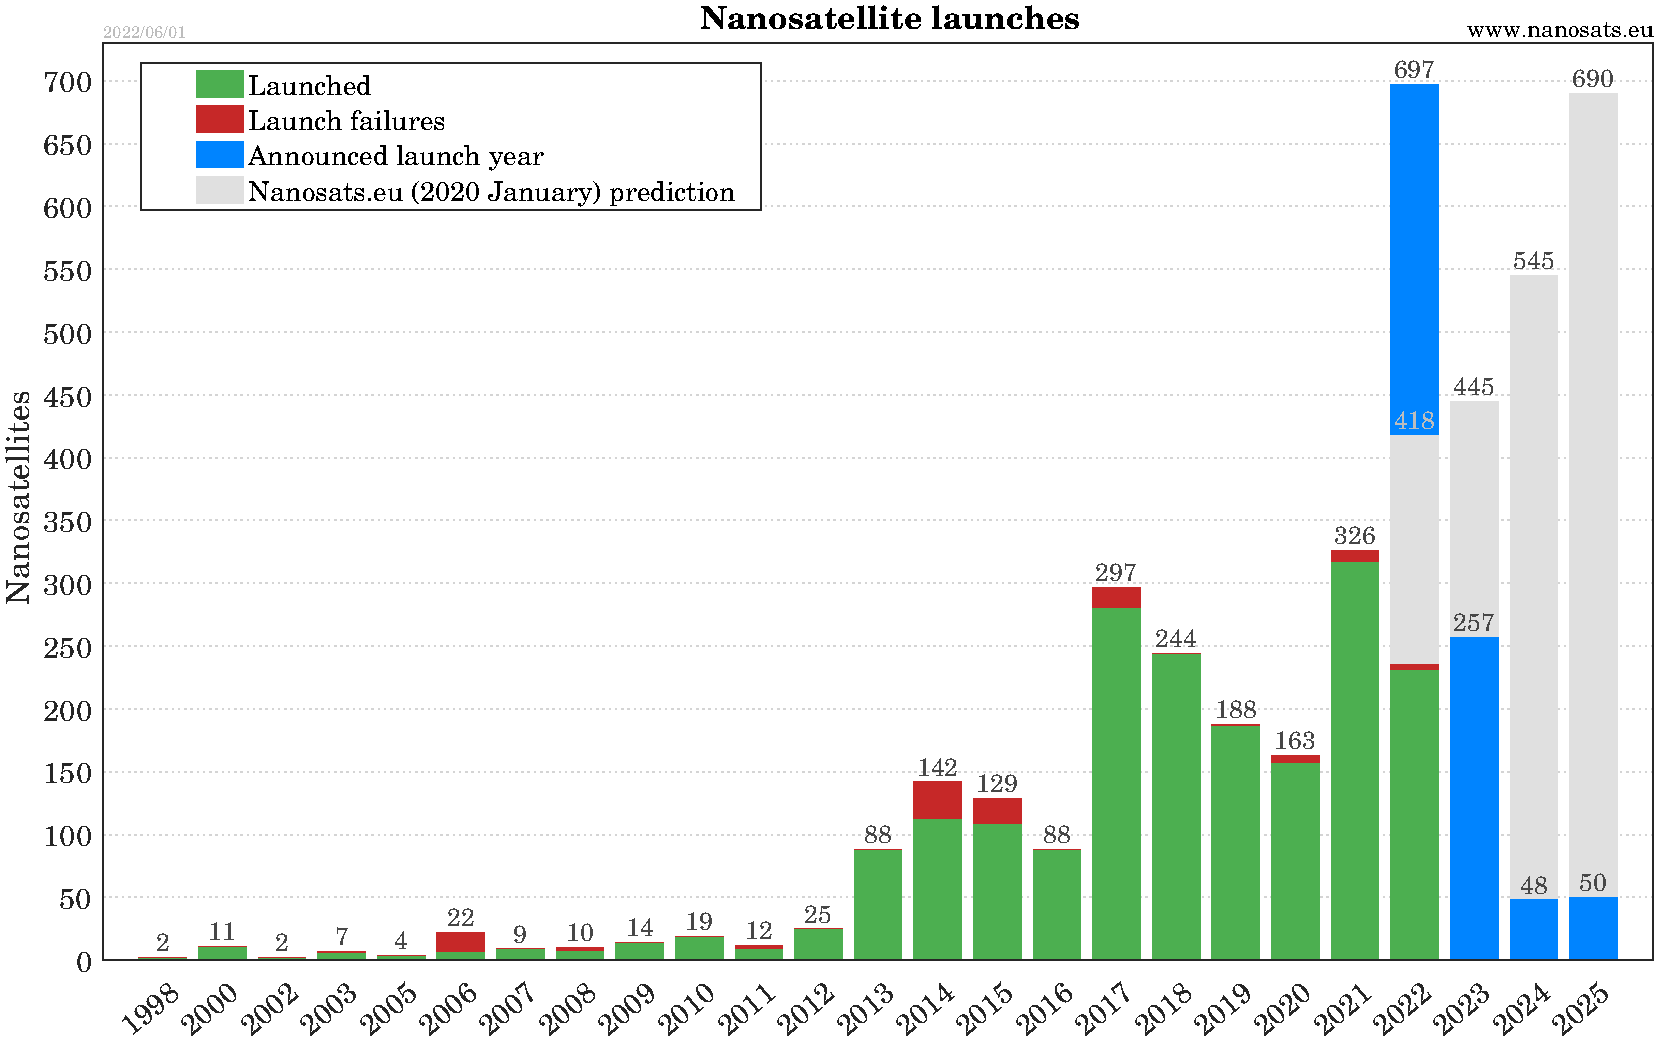
\includegraphics[width=\columnwidth]{figures/Nanosats_years_2022-06-01}
        \caption{Nanosatellite launches (2022/06/01) \cite{nanosatseu}.}
        \label{fig:cubesat-launches}
    \end{center}
\end{figure}

Com um custo consideravelmente menor, devido principalmente a utilização de órbitas mais baixas do tipo LEO\nomenclature{\textbf{LEO}}{Low Earth Orbit} (Low Earth Orbit) e de componentes COTS\nomenclature{\textbf{COTS}}{Commercial Off-The-Shelf}, vem se tornando cada vez mais fácil desenvolver e colocar um satélite em operação no espaço.

Um padrão que dominou o mercado de nanossatélites é o padrão CubeSat \cite{cds}, que normatiza várias características físicas para esses tipos de satélites. Este padrão, além de padronizar os subsistemas espaciais disponíveis no mercado, também normatiza os lançadores, o que faz com que se reduza o custo de lançamento de um nanossatélite, sendo um dos maios custos dentro deste tipo de projeto.

\section{Constellations}

\begin{figure}[!ht]
    \begin{center}
        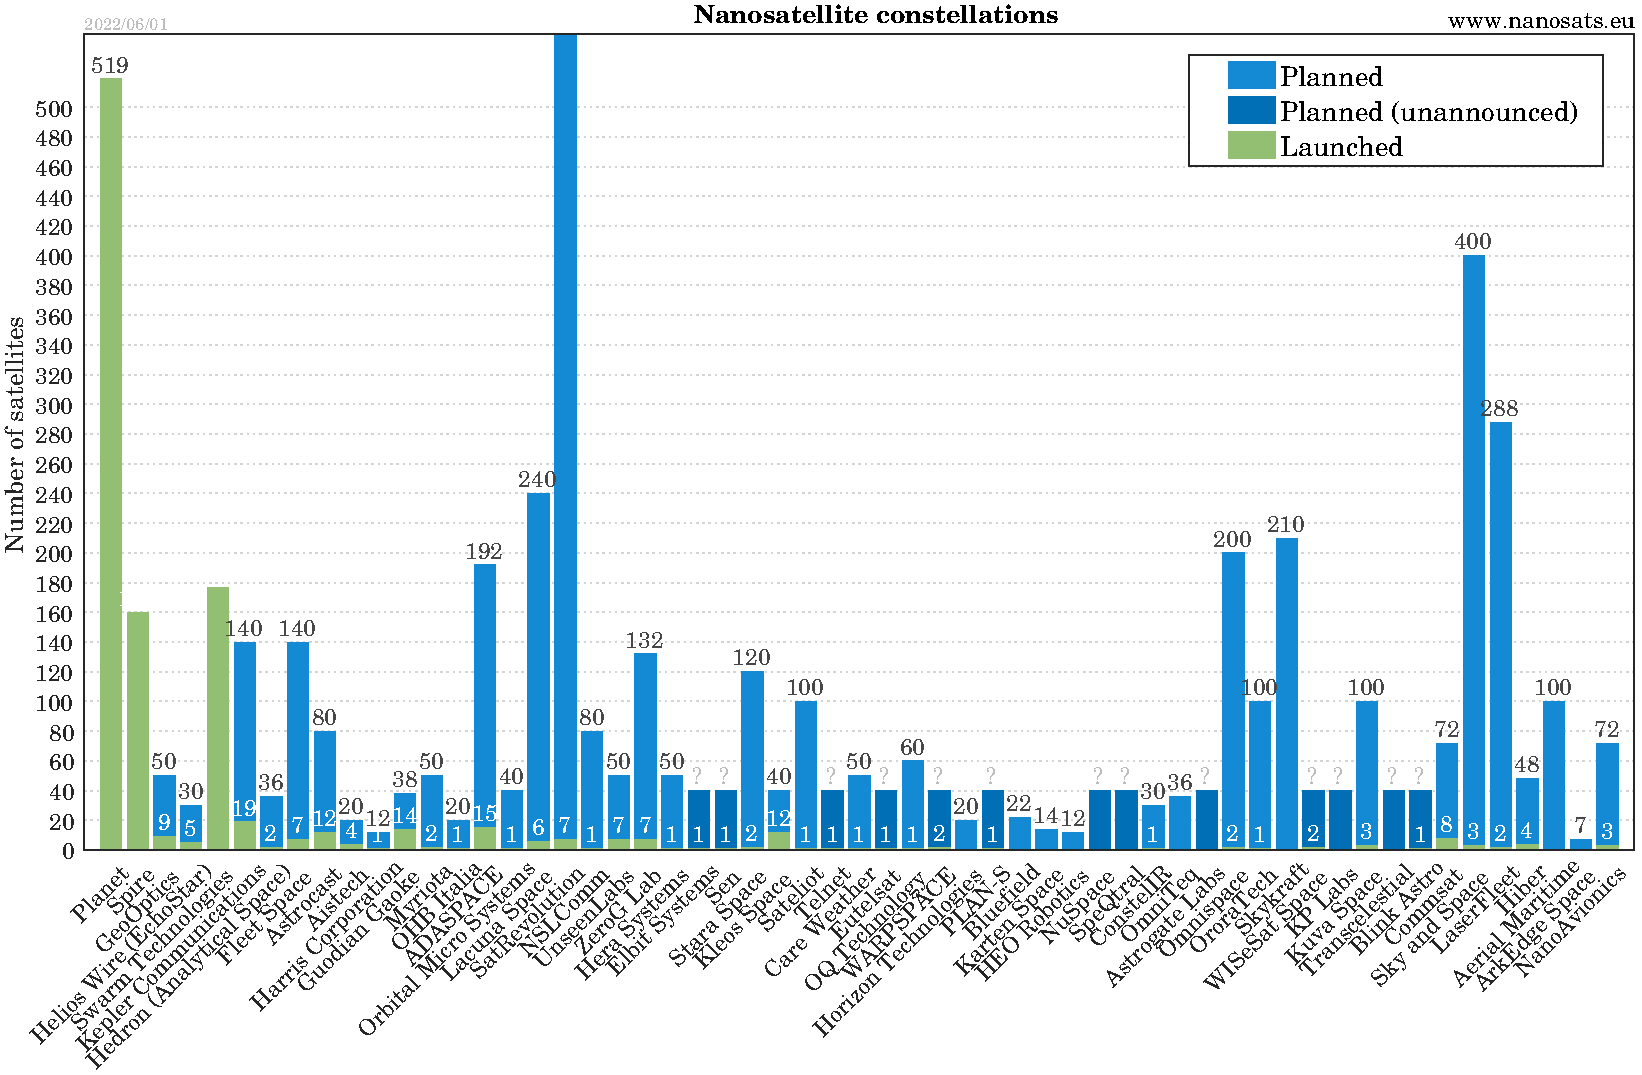
\includegraphics[width=\columnwidth]{figures/Nanosats_constellations_2022-06-01}
        \caption{Nanosatellite constellations (2022/06/01) \cite{nanosatseu}.}
        \label{fig:constellations}
    \end{center}
\end{figure}

\section{Motivation}

.
